% ==============================================================================
% Chapter 5: High-Level Design
% ==============================================================================
\chapter{High-Level Design}
\label{ch:high_level_design}

This chapter articulates the structural and behavioural design of VendorMap through formal architectural models, including the relational Entity-Relationship Diagram (ERD), Data Flow Diagrams (Level 0 and Level 1), and complete Unified Modeling Language (UML) specifications (Use Case, Service Class Architecture, Sequence, and Activity diagrams).

\section{Entity Relationship Diagram (ERD)}
\label{sec:erd}

The operational persistence layer is implemented in SQLite using SQLAlchemy Core abstraction. The schema strictly decouples operational transaction management from research model artifacts. Fig.~\ref{fig:erd_diagram} depicts the Entity-Relationship Diagram modeling the core database entities, primary/foreign key relationships, and structural cardinality.

\begin{figure*}[htbp]
\centering
\begin{tikzpicture}[
    node distance=1.6cm and 1.8cm,
    entity/.style={
        rectangle, draw=blue!70, fill=blue!5, rounded corners=2pt,
        font=\scriptsize, inner sep=4pt, text width=3.4cm
    },
    header/.style={
        font=\scriptsize\bfseries, fill=blue!15, text centered, draw=blue!70
    },
    rel/.style={
        draw=black!70, thick, -{Latex[length=2mm]}
    },
    carrow/.style={
        draw=black!75, thick
    }
]

% Operational Entities
\node[entity] (vendor) {
    \textbf{operational\_vendors}\\
    \hrulefill\\
    \underline{vendor\_id} (PK)\\
    application\_vendor\_id\\
    vendor\_type\\
    full\_name, business\_name\\
    business\_category\\
    preferred\_division\\
    priority\_profile\\
    preferred\_language\\
    status, created\_at
};

\node[entity, right=1.6cm of vendor] (zone) {
    \textbf{zone\_live\_status}\\
    \hrulefill\\
    \underline{zone\_id} (PK)\\
    official\_capacity\\
    current\_vendor\_count\\
    available\_capacity\\
    status (OPEN/FULL/etc.)\\
    verified\_at, verified\_by\\
    updated\_at
};

\node[entity, below=1.2cm of vendor] (auth_ident) {
    \textbf{vendor\_auth\_identities}\\
    \hrulefill\\
    \underline{identity\_id} (PK)\\
    vendor\_id (FK)\\
    phone\_hash (HMAC-SHA256)\\
    vendor\_source\\
    is\_verified\\
    created\_at
};

\node[entity, below=1.2cm of zone] (alloc_req) {
    \textbf{allocation\_requests}\\
    \hrulefill\\
    \underline{request\_id} (PK)\\
    vendor\_id (FK)\\
    zone\_id (FK)\\
    request\_type (NEW/RELOC)\\
    status (PENDING/APP/REJ)\\
    reviewed\_at, reviewed\_by\\
    rejection\_reason, notes
};

\node[entity, below=1.2cm of alloc_req] (alloc) {
    \textbf{allocations}\\
    \hrulefill\\
    \underline{allocation\_id} (PK)\\
    vendor\_id (FK)\\
    zone\_id (FK)\\
    request\_id (FK)\\
    status (ACTIVE/RELEASED)\\
    allocated\_at, released\_at
};

\node[entity, right=1.6cm of zone] (pilot_layout) {
    \textbf{pilot\_slot\_layouts}\\
    \hrulefill\\
    \underline{zone\_id} (PK / FK)\\
    metadata\_json\\
    created\_at
};

\node[entity, below=1.2cm of pilot_layout] (pilot_slot) {
    \textbf{pilot\_slots}\\
    \hrulefill\\
    \underline{zone\_id, slot\_id} (PK)\\
    width\_m, depth\_m\\
    x\_m, y\_m\\
    geometry\_json (EPSG:4326)\\
    status (AVAIL/OCC/BLOCK)\\
    assigned\_vendor\_id (FK)\\
    updated\_at
};

\node[entity, below=1.2cm of auth_ident] (sessions) {
    \textbf{auth\_sessions}\\
    \hrulefill\\
    \underline{session\_id} (PK)\\
    session\_token\_hash\\
    role (VENDOR/ADMIN)\\
    vendor\_id / admin\_id\\
    expires\_at, revoked\_at
};

\node[entity, right=1.6cm of alloc] (audit) {
    \textbf{admin\_audit\_log}\\
    \hrulefill\\
    \underline{audit\_id} (PK)\\
    action, entity\_type\\
    entity\_id, performed\_by\\
    details\_json\\
    created\_at
};

% Connectors
\draw[rel] (auth_ident.north) -- node[left, font=\tiny] {1:1} (vendor.south);
\draw[rel] (sessions.north) -- (auth_ident.south);
\draw[rel] (alloc_req.west) -- node[above, font=\tiny] {N:1} (vendor.east);
\draw[rel] (alloc_req.north) -- node[right, font=\tiny] {N:1} (zone.south);
\draw[rel] (alloc.north) -- (alloc_req.south);
\draw[rel] (pilot_layout.south) -- node[right, font=\tiny] {1:N} (pilot_slot.north);
\draw[rel] (zone.east) -- node[above, font=\tiny] {1:1} (pilot_layout.west);
\draw[rel] (alloc.east) -- (audit.west);
\draw[rel] (pilot_slot.west) -- node[below, font=\tiny] {0..1} (alloc.north east);

\end{tikzpicture}
\caption{Entity-Relationship Diagram (ERD) of the VendorMap operational database schema.}
\label{fig:erd_diagram}
\end{figure*}

\section{Data Flow Diagrams (DFD)}
\label{sec:dfd}

\subsection{Level 0 DFD (Context Diagram)}
Fig.~\ref{fig:dfd_level0} illustrates the Level 0 Context Diagram of VendorMap, depicting the external entities interacting across system boundaries.

\begin{figure}[htbp]
\centering
\begin{tikzpicture}[
    node distance=2.2cm,
    ext/.style={
        rectangle, draw=black!80, fill=gray!12, rounded corners=2pt,
        font=\small\bfseries, text centered, inner sep=6pt, text width=2.6cm
    },
    proc/.style={
        circle, draw=blue!75, fill=blue!10, line width=1pt,
        font=\small\bfseries, text centered, inner sep=6pt, text width=3.2cm
    },
    arrow/.style={
        ->, >=stealth, thick, draw=black!75
    }
]

\node[proc] (system) {0.0\\VendorMap\\Municipal System};

\node[ext, above=1.8cm of system] (officer) {NMC Town-Planning\\Officer (Admin)};
\node[ext, below=1.8cm of system] (vendor) {Street Vendor\\(Web / WhatsApp)};
\node[ext, left=2.2cm of system] (osm) {OpenStreetMap\\Spatial Services};
\node[ext, right=2.2cm of system] (meta) {Meta WhatsApp\\Cloud API Gateway};

\draw[arrow] (officer) -- node[left, font=\scriptsize] {AHP Matrix, Capacities, Approvals} (system);
\draw[arrow] (system) -- node[right, font=\scriptsize] {GIS Maps, Audit Logs, Allocation Plans} (officer);

\draw[arrow] (vendor) -- node[left, font=\scriptsize] {OTP, Profile, Relocation Request} (system);
\draw[arrow] (system) -- node[right, font=\scriptsize] {Recommendations, Assigned Slot, Route} (vendor);

\draw[arrow] (osm) -- node[above, font=\scriptsize] {Road Vectors, POIs} (system);
\draw[arrow] (meta) -- node[above, font=\scriptsize] {Webhook Inbound} (system);
\draw[arrow] (system) -- node[below, font=\scriptsize] {Outbound Messages} (meta);

\end{tikzpicture}
\caption{Level 0 Context Data Flow Diagram (DFD) of VendorMap.}
\label{fig:dfd_level0}
\end{figure}

\subsection{Level 1 DFD (Decomposed Processes)}
Fig.~\ref{fig:dfd_level1} decomposes the system into six core operational processes and five internal data repositories.

\begin{figure*}[htbp]
\centering
\begin{tikzpicture}[
    node distance=1.4cm and 1.4cm,
    proc/.style={
        circle, draw=blue!70, fill=blue!8,
        font=\scriptsize\bfseries, text centered, inner sep=3pt, text width=2.4cm
    },
    store/.style={
        rectangle, draw=black!70, fill=yellow!10, dashed,
        font=\scriptsize, inner sep=4pt, text width=2.4cm, text centered
    },
    ext/.style={
        rectangle, draw=black!80, fill=gray!12,
        font=\scriptsize\bfseries, text centered, inner sep=4pt, text width=2.0cm
    },
    arrow/.style={
        ->, >=stealth, thick, draw=black!70
    }
]

% External entities
\node[ext] (ext_vendor) {Street Vendor};
\node[ext, right=7.0cm of ext_vendor] (ext_admin) {NMC Officer};

% Processes
\node[proc, below=1.0cm of ext_vendor] (p1) {1.0\\Authentication\\\& OTP Hashing};
\node[proc, right=1.4cm of p1] (p2) {2.0\\Spatial MCDA\\Recommendation};
\node[proc, right=1.4cm of p2] (p3) {3.0\\Goal Programming\\Batch Optimizer};
\node[proc, below=1.8cm of p1] (p4) {4.0\\Relocation Request\\Lifecycle};
\node[proc, below=1.8cm of p2] (p5) {5.0\\Micro-Slot Packing\\\& Navigation};
\node[proc, below=1.8cm of p3] (p6) {6.0\\Audit Logging\\\& Enforcement};

% Data stores
\node[store, below=0.8cm of p4] (d1) {\textbf{D1} Vendor Registry};
\node[store, right=1.4cm of d1] (d2) {\textbf{D2} Zone Capacity DB};
\node[store, right=1.4cm of d2] (d3) {\textbf{D3} Pilot Slot Layouts};

% Flows
\draw[arrow] (ext_vendor) -- (p1);
\draw[arrow] (p1) -- (d1);
\draw[arrow] (p1) -- (p2);
\draw[arrow] (p2) -- (d2);
\draw[arrow] (p2) -- (p4);
\draw[arrow] (p4) -- (p3);
\draw[arrow] (ext_admin) -- (p3);
\draw[arrow] (p3) -- (d2);
\draw[arrow] (p3) -- (p5);
\draw[arrow] (p5) -- (d3);
\draw[arrow] (p5) -- node[left, font=\tiny] {Walking Route} (ext_vendor);
\draw[arrow] (p3) -- (p6);
\draw[arrow] (p4) -- (p6);

\end{tikzpicture}
\caption{Level 1 Data Flow Diagram (DFD) showing internal processes and operational stores.}
\label{fig:dfd_level1}
\end{figure*}

\section{UML Diagrams}
\label{sec:uml_diagrams}

\subsection{Use Case Diagram}
Fig.~\ref{fig:uml_usecase} details the system Use Case Diagram, categorizing actions available to Street Vendors, Town-Planning Officers, and the Meta WhatsApp Cloud API gateway.

\begin{figure}[htbp]
\centering
\begin{tikzpicture}[
    actor/.style={
        rectangle, draw=black!70, fill=blue!5, rounded corners=3pt,
        font=\scriptsize\bfseries, text centered, inner sep=4pt, text width=2.2cm
    },
    usecase/.style={
        ellipse, draw=black!70, fill=green!8,
        font=\scriptsize, text centered, inner sep=2pt, text width=2.8cm, minimum height=0.7cm
    },
    arrow/.style={
        -, thick, draw=black!70
    }
]

% Actors
\node[actor] (act_vendor) {Street Vendor};
\node[actor, below=4.0cm of act_vendor] (act_admin) {Town-Planning\\Officer (Admin)};

% Boundary box
\draw[dashed, black!40, rounded corners=6pt] (3.0, 1.2) rectangle (10.0, -6.5);
\node[font=\footnotesize\bfseries, color=black!60] at (6.5, 0.8) {VendorMap System Boundary};

% Use cases
\node[usecase] (uc1) at (6.5, 0.0) {Authenticate via Mobile OTP (HMAC)};
\node[usecase] (uc2) at (6.5, -1.0) {Query Personalized Zone Recommendations};
\node[usecase] (uc3) at (6.5, -2.0) {Submit Relocation / Allocation Request};
\node[usecase] (uc4) at (6.5, -3.0) {Navigate to Designated Slot (Leaflet GPS)};
\node[usecase] (uc5) at (6.5, -4.0) {Review \& Execute Batch Allocations (MILP)};
\node[usecase] (uc6) at (6.5, -5.0) {Demarcate Micro-Slots \& Corridors};
\node[usecase] (uc7) at (6.5, -6.0) {Calibrate AHP Criteria Weights};

% Connections
\draw[arrow] (act_vendor) -- (uc1);
\draw[arrow] (act_vendor) -- (uc2);
\draw[arrow] (act_vendor) -- (uc3);
\draw[arrow] (act_vendor) -- (uc4);

\draw[arrow] (act_admin) -- (uc1);
\draw[arrow] (act_admin) -- (uc5);
\draw[arrow] (act_admin) -- (uc6);
\draw[arrow] (act_admin) -- (uc7);

\end{tikzpicture}
\caption{UML Use Case Diagram representing primary actors and system capabilities.}
\label{fig:uml_usecase}
\end{figure}

\subsection{Service Architecture / Class Diagram}
VendorMap follows a service-oriented architectural pattern in Python. Fig.~\ref{fig:uml_class} illustrates the core domain services, repositories, and mathematical engines.

\begin{figure*}[htbp]
\centering
\begin{tikzpicture}[
    classbox/.style={
        rectangle, draw=blue!75, fill=blue!4, rounded corners=2pt,
        font=\scriptsize, inner sep=4pt, text width=4.2cm
    },
    arrow/.style={
        draw=black!75, thick, -{Latex[length=2mm]}
    }
]

\node[classbox] (repo) {
    \textbf{DatabaseRepository}\\
    \hrulefill\\
    - engine: Engine\\
    - metadata: MetaData\\
    \hrulefill\\
    + get\_vendor(vendor\_id): Vendor\\
    + list\_zones(status): List[Zone]\\
    + create\_request(req): Request\\
    + commit\_allocation(alloc): void\\
    + log\_audit(action, entity): void
};

\node[classbox, right=1.6cm of repo] (mcda) {
    \textbf{MCDAEngine}\\
    \hrulefill\\
    - weights: Dict[str, float]\\
    - scales: Dict[str, float]\\
    \hrulefill\\
    + compute\_suitability(v, z): float\\
    + apply\_shrinkage(c, z): float\\
    + rank\_candidates(v, pool): List\\
    + explain\_score(v, z): Dict
};

\node[classbox, below=1.2cm of repo] (geom) {
    \textbf{PilotGeometryEngine}\\
    \hrulefill\\
    - crs\_metric: CRS (EPSG:32643)\\
    - slot\_dim: Tuple[float, float]\\
    \hrulefill\\
    + project\_polygon(geom): Polygon\\
    + generate\_slots(poly, count): List\\
    + validate\_corridor(poly, slots): bool\\
    + reproject\_wgs84(slots): GeoJSON
};

\node[classbox, below=1.2cm of mcda] (milp) {
    \textbf{AllocationOptimizer}\\
    \hrulefill\\
    - solver: HiGHS (scipy.milp)\\
    - penalties: Dict[str, float]\\
    \hrulefill\\
    + solve\_cardinality(V, Z): int\\
    + solve\_quality(V, Z, U*): Plan\\
    + audit\_capacities(Plan): bool
};

\draw[arrow] (mcda) -- node[above, font=\tiny] {Reads zones/vendors} (repo);
\draw[arrow] (milp) -- node[right, font=\tiny] {Suitability Matrix} (mcda);
\draw[arrow] (milp) -- node[above, font=\tiny] {Commits Plan} (repo);
\draw[arrow] (geom) -- node[left, font=\tiny] {Persists Slots} (repo);

\end{tikzpicture}
\caption{UML Service Architecture and Class Diagram illustrating service relationships.}
\label{fig:uml_class}
\end{figure*}

\subsection{Sequence Diagram}
Fig.~\ref{fig:uml_sequence} details the interaction sequence when an authenticated vendor queries zone recommendations and submits a relocation request for municipal officer approval.

\begin{figure*}[htbp]
\centering
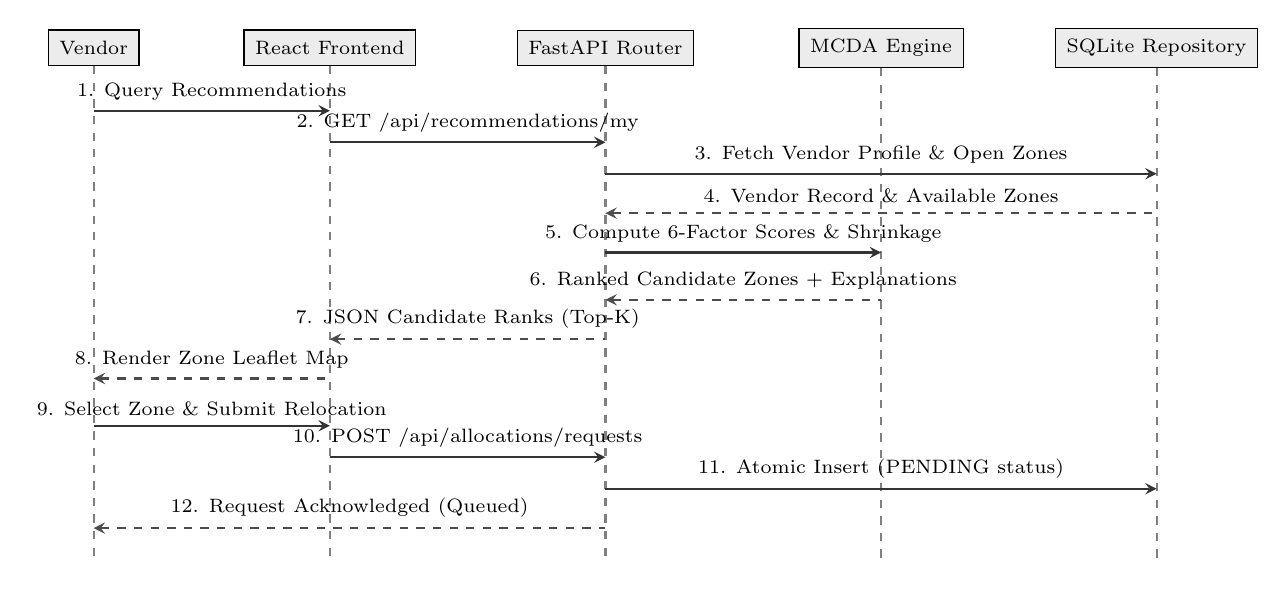
\begin{tikzpicture}[
    font=\scriptsize,
    lifeline/.style={draw=black!50, dashed, thick},
    activation/.style={draw=blue!70, fill=blue!10, rectangle, inner sep=0pt},
    msg/.style={->, >=stealth, thick, draw=black!80},
    ret/.style={<-, >=stealth, dashed, thick, draw=black!70}
]

% Participants
\node[rectangle, draw=black, fill=gray!15, inner sep=4pt] (p_ven) at (0, 0) {Vendor};
\node[rectangle, draw=black, fill=gray!15, inner sep=4pt] (p_ui) at (3.0, 0) {React Frontend};
\node[rectangle, draw=black, fill=gray!15, inner sep=4pt] (p_api) at (6.5, 0) {FastAPI Router};
\node[rectangle, draw=black, fill=gray!15, inner sep=4pt] (p_mcda) at (10.0, 0) {MCDA Engine};
\node[rectangle, draw=black, fill=gray!15, inner sep=4pt] (p_db) at (13.5, 0) {SQLite Repository};

% Lifelines
\draw[lifeline] (p_ven) -- (0, -6.5);
\draw[lifeline] (p_ui) -- (3.0, -6.5);
\draw[lifeline] (p_api) -- (6.5, -6.5);
\draw[lifeline] (p_mcda) -- (10.0, -6.5);
\draw[lifeline] (p_db) -- (13.5, -6.5);

% Messages
\draw[msg] (0, -0.8) -- node[above] {1. Query Recommendations} (3.0, -0.8);
\draw[msg] (3.0, -1.2) -- node[above] {2. GET /api/recommendations/my} (6.5, -1.2);
\draw[msg] (6.5, -1.6) -- node[above] {3. Fetch Vendor Profile \& Open Zones} (13.5, -1.6);
\draw[ret] (6.5, -2.1) -- node[above] {4. Vendor Record \& Available Zones} (13.5, -2.1);
\draw[msg] (6.5, -2.6) -- node[above] {5. Compute 6-Factor Scores \& Shrinkage} (10.0, -2.6);
\draw[ret] (6.5, -3.2) -- node[above] {6. Ranked Candidate Zones + Explanations} (10.0, -3.2);
\draw[ret] (3.0, -3.7) -- node[above] {7. JSON Candidate Ranks (Top-K)} (6.5, -3.7);
\draw[ret] (0, -4.2) -- node[above] {8. Render Zone Leaflet Map} (3.0, -4.2);

\draw[msg] (0, -4.8) -- node[above] {9. Select Zone \& Submit Relocation} (3.0, -4.8);
\draw[msg] (3.0, -5.2) -- node[above] {10. POST /api/allocations/requests} (6.5, -5.2);
\draw[msg] (6.5, -5.6) -- node[above] {11. Atomic Insert (PENDING status)} (13.5, -5.6);
\draw[ret] (0, -6.1) -- node[above] {12. Request Acknowledged (Queued)} (6.5, -6.1);

\end{tikzpicture}
\caption{UML Sequence Diagram detailing the vendor relocation recommendation and request workflow.}
\label{fig:uml_sequence}
\end{figure*}

\subsection{Activity Diagram}
Fig.~\ref{fig:uml_activity} depicts the Activity Diagram capturing the complete operational lifecycle from vendor profile onboarding to physical micro-slot assignment.

\begin{figure}[htbp]
\centering
\begin{tikzpicture}[
    node distance=1.1cm,
    startstop/.style={circle, draw=black, fill=black, inner sep=3pt},
    endstop/.style={circle, draw=black, double, fill=black, inner sep=2.5pt},
    act/.style={
        rectangle, draw=blue!70, fill=blue!8, rounded corners=3pt,
        font=\scriptsize, text centered, inner sep=4pt, text width=5.5cm
    },
    dec/.style={
        diamond, draw=red!70, fill=red!8, font=\tiny\bfseries,
        inner sep=1.5pt, aspect=1.8, text centered
    },
    arrow/.style={->, >=stealth, thick, draw=black!75}
]

\node[startstop] (start) {};
\node[act, below=0.6cm of start] (a1) {Vendor submits mobile number (E.164)};
\node[act, below=0.6cm of a1] (a2) {System hashes number via HMAC-SHA256 \& dispatches OTP};
\node[dec, below=0.6cm of a2] (d1) {OTP Valid?};
\node[act, below=0.6cm of d1] (a3) {Issue HttpOnly Session Cookie \& Load Profile};
\node[act, below=0.6cm of a3] (a4) {Execute MCDA Suitability Scoring across candidate zones};
\node[act, below=0.6cm of a4] (a5) {Vendor selects preferred zone \& submits relocation request};
\node[act, below=0.6cm of a5] (a6) {Town-Planning Officer reviews batch via HiGHS Goal Program};
\node[dec, below=0.6cm of a6] (d2) {Approved?};
\node[act, below=0.6cm of d2] (a7) {Assign metric $2\,\text{m}\times 2\,\text{m}$ slot \& generate walking navigation};
\node[act, right=1.2cm of d2, text width=2.4cm] (a_rej) {Notify rejection with civic reason};
\node[endstop, below=0.6cm of a7] (stop) {};

\draw[arrow] (start) -- (a1);
\draw[arrow] (a1) -- (a2);
\draw[arrow] (a2) -- (d1);
\draw[arrow] (d1) -- node[right, font=\tiny] {Yes} (a3);
\draw[arrow] (d1.east) -- ++(1.2,0) |- node[right, font=\tiny] {No (Retry)} (a1.east);
\draw[arrow] (a3) -- (a4);
\draw[arrow] (a4) -- (a5);
\draw[arrow] (a5) -- (a6);
\draw[arrow] (a6) -- (d2);
\draw[arrow] (d2) -- node[right, font=\tiny] {Yes} (a7);
\draw[arrow] (d2) -- node[above, font=\tiny] {No} (a_rej);
\draw[arrow] (a7) -- (stop);

\end{tikzpicture}
\caption{UML Activity Diagram for vendor registration, relocation evaluation, and slot allocation.}
\label{fig:uml_activity}
\end{figure}
